\newpage
\usecasebase{Visualizzazione notifica risposta \textit{feedback}}
\label{usecase:Visualizzazione notifica risposta feedback}

\begin{figure}[h]
	\centering
	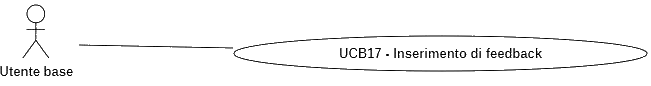
\includegraphics[width=0.8\textwidth]{./uml/UCB17.png} 
	\caption{Visualizzazione notifica risposta \textit{feedback}}
	\label{fig:UCB19}
  \end{figure}

\begin{itemize}
	\item \textbf{Attore principale:} Utente base.

	\item \textbf{Precondizione:} L'Utente ristoratore ha risposto ad un determinato \textit{feedback} (vedi \autoref{usecase:Risposta ad un feedback}).


	\item \textbf{Postcondizione:} L'Utente base visualizza la notifica relativamente ad un suo \textit{feedback}, che ha ricevuto risposta da parte del ristoratore.

	\item \textbf{Scenario principale:}
	      \begin{enumerate}
		      \item Il Sistema rivela l'inserimento di una risposta da parte del ristoratore;

		      \item Il Sistema invia una notifica all'Utente base, autore del \textit{feedback}, che ha ricevuto risposta da parte del ristoratore.
	      \end{enumerate}
\end{itemize}
